
\documentclass{standalone}
\usepackage{tikz}
\usepackage{pgfplots}
\usetikzlibrary{calc}
\begin{document}

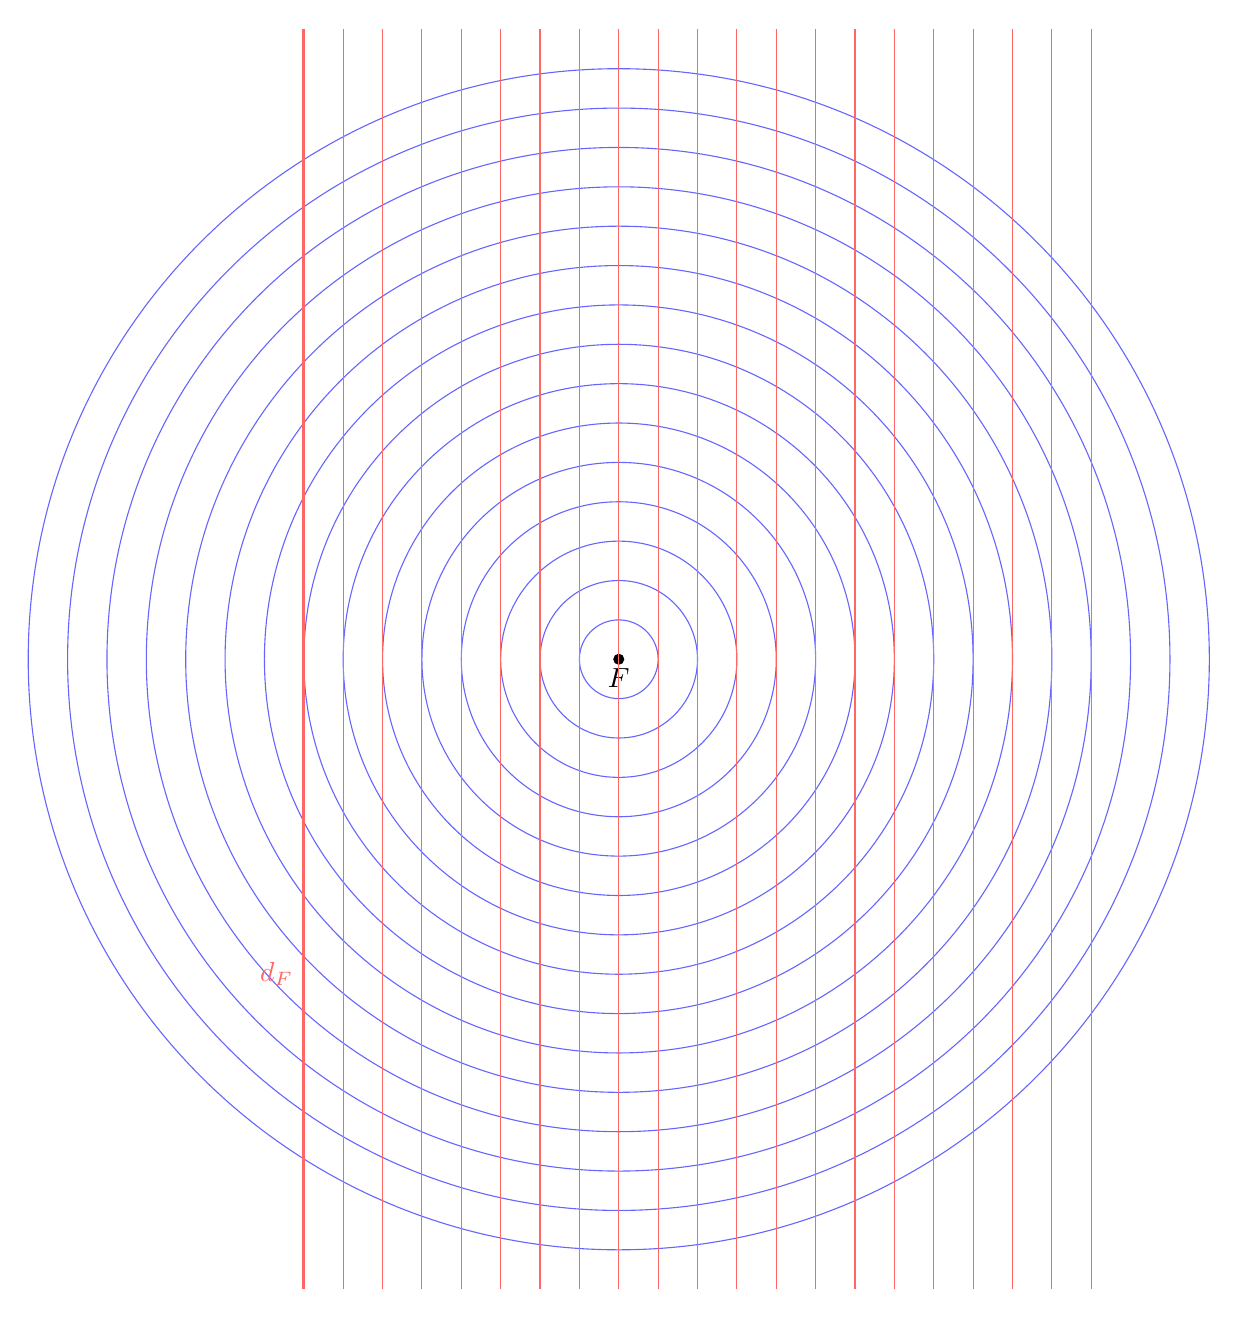
\begin{tikzpicture}[scale=1]

% Points F1 and F2
\coordinate (F1) at (-2,0);
\coordinate (F2) at (-6,0);

% Draw the points
\fill (F1) circle (2pt) node[below] {$F$};
%\fill (F2) circle (2pt) node[below] {$F_2$};

% Circles centered at F1
\foreach \r in {1,2,...,15}
{
    \draw[blue!60] (F1) circle (\r*0.5);
}

% Vertical lines centered at F2
\draw[red!60, very thick] ($(F2)+(0,-8)$) -- ($(F2)+(0,8)$) node[near start, left] {$d_F$};
\foreach \i in {0,...,20}
{
    % x offset for each line (0.5 spacing like the circles)
    \pgfmathsetmacro{\x}{0 + 0.5*\i}
    % Draw vertical line from bottom to top
    \draw[red!60] ($(F2)+(\x,-8)$) -- ($(F2)+(\x,8)$);
}

\end{tikzpicture}
\end{document}